\documentclass{article}

\usepackage[utf8]{inputenc}
\usepackage[spanish]{babel}
\usepackage{ragged2e}

\usepackage{graphicx}
\graphicspath{ {./imagenes/} }

\usepackage{geometry}
\geometry{margin=3cm}

\title{Historia de la computación en México de los últimos 50 años}
\author{Axel Treviño Palacios} 
\date{2020-21-10}

\begin{document}
\maketitle

Un hombre con mucha presencia dentro de la computación en México es el profesor Harold B. McIntosh (1929-2015), quien, con ayuda de otros, la impulsó de gran manera y concretó su existencia dentro del país. 

Inició sus aportaciones a la intitución en 1965, cuando ayudó a fundar la Maestría en Computacion en el Centro Nacional de Cálculo (primera de su tipo en America Latina).

Después, entre 1966 y 1975, enseñó como profesor en la Escuela Superior de Fisica y Matemáticas (ESFM), periodo durante también actuó como coordinador de la Academia de Matemáticas Aplicadas.

El curso que impartía pivotaba al rededor de la lógica matemática, y se alternaba entre prácticas de programación con la PDP-8 y las clases teóricas sobre Álgebra Booleana. Esto propiciaba el desarrollo contiguo de las habilidades de programación y de los conocimientos sobre teoría computacional dentro de la mente de los estudiantes.

Para poder procesar de mejor manera los algoritmos de Markov, McIntosh propuso dearrollar una imitacion de REC (un lenguaje educacional con la capacidad de usar estructuras de datos recursivas) llamada REC/Markov.

Uno de los principales objetivos de la compra de una PDP-10 dentro de la INEN fué el estudio de minerales, para lo cual se desarrolló el conjunto de subrutinas llamado PLOT, al cual le fueron añadiendo otros paquetes, como PHOC (Plane Homogeneous Coordinates) y SHOC (Space Homogenous Coordinates).

La primera computadora electronica en México fué una IBM 650, instalada en la UNAM en junio de 1958. Los responsables de ello fueron:

\begin{itemize}
	\item Nabor Carrill, rector en ese entonces de la UNAM
	\item Alberto Barajas, director de Ciencias
	\item Carlos Graef, decano de la Facultad de Ciencias
	\item Sergio Beltran, líder del grupo de investigación en la Facultad de Ingeniería
\end{itemize}

Como en ese entonces no muchas personas sabían cómo utilizar una computadora electrónica, éste último organizó y fundó el Centro de Computación de la UNAM, con el fin de entrenar a los estudiantes que lo necesitaran, y fué seleccionado como su primer director.

Los avances de tecnología y ciencias de México fueron realizados desde cero, lo cual propició una desconexión entre los grupos de investigación (los dos principales residiendo en la UNAM y en la UAP, y otros pequeños desperdigados por todo el país). Esto no ayudó el estado de investigación del país cuando ocurrió la recesión económica de 1982, porque ésta area fué la primera en sufrir recortes de presupuesto, disminuyendo el número de investigadores de 22 a 4 por 1984.

Esta mentalidad no se ha movido desde entonces, colocando la importancia del desarrollo científico y tecnológico del país en un nivel deplorablemente bajo, recurriendo a importar tecnologías que no poseamos en vez de desarrollarlas, favoreciendo el estancamiento del conocimiento científico dentro del país. A pesar de todo esto, el campo académico de computación ha crecido constantemente desde los años ochenta.

Durante la década de los noventas nuestro país tuvo numerosas contribuciones a distintas areas de la ciencia de computación, dentro de las cuales estuvo a segunda etapa de las aportaciones de McIntosh: la teoría del autómata celular. Durante este tiempo, McIntosh discutió dentro de sus cátedras sus pensamientos sobre el problema del uso de las supercomputadoras en medios no lineares, perteneciente a esta teoría. Todas estas palabras y conocimientos fueron compendiados en su libro "One Dimensional Cellular Automata", publicado en 2009.

Uno de los problemas a los que dedicó sus últimos años fué la idea de un autómata celular reversible. Empezó a ponderar sobre ello desde inicios de los años noventa, para lo cual recibió ayuda de un grupo de estudaintes de la Academia Mexicana de Ciencia (AMS).

La inteligencia de McIntosh es tal que logra cruzar epocas temporales al aún ser pertinente en nuestros tiempos, alcanzando incluso temas ajenos al desciframiento de las propiedades de los autómatas celulares reversibles, como la clasificación de los comportamientos de autómatas celulares elementales o la aplicación de los autómatas celulares a una simulación de un sistema de manufacturación.

\pagebreak
\begin{center}
	\textbf{Grafo de Autómata de cadenas binarias}
	
	Autómata que reconoce cadenas binarias con numeros impares de unos y ceros:
	\begin{figure}[h]
		\centering

		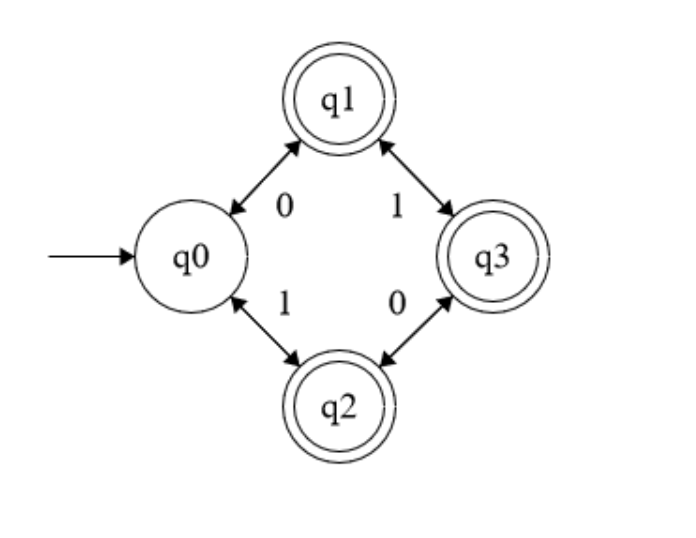
\includegraphics[width=15cm]{grafo}
		\caption{Grafo}
	\end{figure}	
\end{center}




\end{document}